\section{Auswertung}
\label{sec:Auswertung}

\subsection{Ermittlung der effekiven Reichweite und der Energie der Alpha-Teilchen}
Aus dem Druck und dem Abstand des Detektors zur Quelle wird mit Gleichung 4 die effekive Reichweite $x$ der $\alpha$-Teilchen bestimmt. 
Die Energie kann man bestimmen, indem angenommen wird, dass die Position des Maximums bei $0$ $\si{\milli\bar}$ einer Energie von 4 $\si{\MeV}$ entspricht und von einer linearen Energsieskala ausgegangen wird.
Alle gemessenen und berechneten Werte sind in Tabelle 1 und 2 für die beiden Abstände aufgelistet.


\begin{table}[H]
  \centering
  \caption{Druck, Channel, Anzahl an gemessenen Impulsen, berechnete Energie und effektive Reichweite der Teilchen für einen Abstand von $1,8$ $\si{\cm}$.}
  \label{tab:Parameter}
  \begin{tabular}{c c c c c}
    \toprule
    $p/$mbar& Channel & $N/$ & $E/$MeV & $x/$cm \\
    \bottomrule
    0 & 520 & 76536 & 4,00 & 0,00 \\
    50 & 487 & 71337 & 3,75 & 0,09 \\
    100 & 472 & 68768 & 3,63 & 0,18 \\
    150 & 463 & 65863 & 3,56 & 0,27 \\
    200 & 440 & 62204 & 3,38 & 0,36 \\
    250 & 419 & 58339 & 3,22 & 0,44 \\
    300 & 448 & 58861 & 3,35 & 0,53 \\
    350 & 440 & 66611 & 3,38 & 0,62 \\
    400 & 431 & 62401 & 3,32 & 0,71 \\
    450 & 408 & 57024 & 3,14 & 0,8 \\
    500 & 399 & 51804 & 3,07 & 0,89 \\
    550 & 384 & 43950 & 2,95 & 0,98 \\
    600 & 384 & 36752 & 2,95 & 1,07 \\
    650 & 384 & 27549 & 2,95 & 1,15 \\
    700 & 384 & 19646 & 2,95 & 1,24 \\
    750 & 379 & 10923 & 2,92 & 1,33 \\
    800 & 380 & 6037 & 2,92 & 1,42 \\
    850 & 378 & 2710 & 2,91 & 1,51 \\
    900 & 379 & 815 & 2,92 & 1,6 \\
    950 & 378 & 393 & 2,91 & 1,69 \\
    1000 & 388 & 84 & 2,98 & 1,78 \\
 
     \bottomrule
  \end{tabular}
\end{table}

\noindent Die Zählrate wir als Funktion der effektiven Weglänge aufgetragen, und für den linearen Teil wird eine lineare Ausgleichsrechnung durchgeführt.
Der Plot ist in Abbildung 2 zu sehen.
\begin{figure}[H]
  \centering
  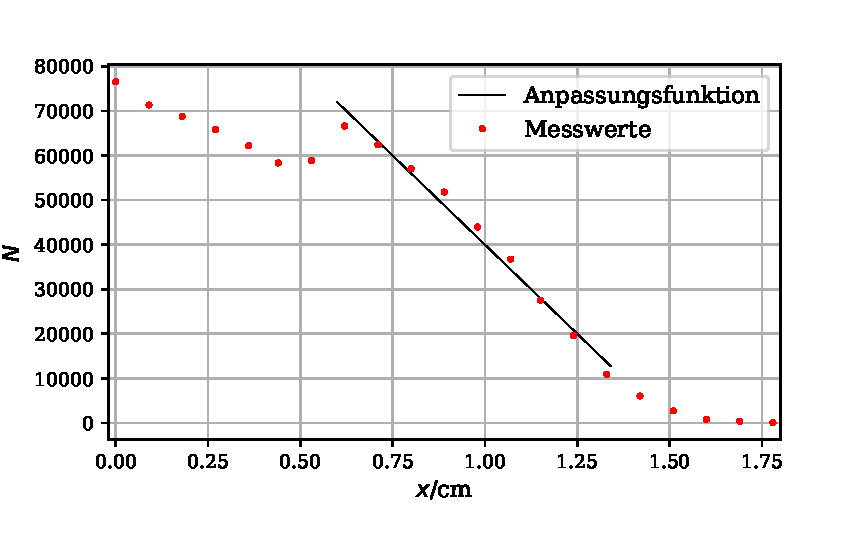
\includegraphics{plot1.pdf}
  \caption{Zählrate in Abhängikeit der effektiven Weglänge für einen Abstand von $1,8$ $\si{\cm}$. }
  \label{fig:plot}
\end{figure}

\noindent Die Parameter der Ausgleichsrechnung der Form $y=ax+b$ lauten
\begin{align*}
a &=  (-79951,82 \pm 3690,95) \frac{1}{\si{\meter}}\\
b &= 119937,39 \pm 3702,19 \\
\end{align*}
Daraus kann die mittlere Reichweite der Teilchen bestimmt werden. Die Zählrate beträgt $N=76536$ und die Hälfte dementsprechend $\frac{N}{2}=38268$. Setzt man dies als y in die Geradengleichung zusammen mit den Parametern ein und löst nach $x$ auf, erhält man
\begin{align*}
R_{m1} = (1,02 \pm 0,07) \si{\meter},
\end{align*}
wobei sich der zugehörige Fehler bestimmen lässt durch die Gaußsche Fehlerfortpflanzung
\begin{align*}
\Delta R_{m} = \sqrt{(\frac{dR_m}{da})^2 (\Delta a)^2 + (\frac{dR_m}{db})^2 (\Delta b)^2}
\end{align*}
mit $\Delta a $ und $\Delta b$ als jeweilige Fehler der Parameter der Ausgleichsgeraden.
Aus dieser Größe wird nun die Energie mit Gleichung 3 bestimmt:
\begin{align*}
E_{1} = (47,7 \pm 2,1) \si{\MeV}.
\end{align*}
Der Fehler kann berechnet werden durch
\begin{align*}
\Delta E = \sqrt{(\frac{dE}{dR_m})^2 (\Delta R_m)^2 }.
\end{align*}


\begin{table}[H]
  \centering
  \caption{Druck, Channel, Anzahl an gemessenen Impulsen, berechnete Energie und effektive Reichweite der Teilchen für einen Abstand von $1,5$ $\si{\cm}$.}
  \label{tab:Parameter}
  \begin{tabular}{c c c c c}
    \toprule
    $p/$mbar& Channel & $N/$ & $E/$MeV & $x/$cm \\
    \bottomrule
    0 & 527 & 100641 & 4,00 & 0,00 \\
    50 & 504 & 99843 & 3,83 & 0,07 \\
    100 & 480 & 97151 & 3,64 & 0,1 \\
    150 & 456 & 89611 & 3,46 & 0,22 \\
    200 & 448 & 81133 & 3,40 & 0,3 \\
    250 & 440 & 80746 & 3,34 & 0,37 \\
    300 & 448 &87899 & 3,40 & 0,44 \\
    350 & 416 & 73592 & 3,16 & 0,52 \\
    400 & 391 & 62289 & 2,97 & 0,59 \\
    450 & 399 & 60611 & 3,03 & 0,67 \\
    500 & 384 & 48074 & 2,91 & 0,74 \\
    550 & 384 & 42297 & 2,91 & 0,81 \\
    600 & 384 & 50444 & 2,91 & 0,89 \\
    650 & 383 & 22476 & 2,91 & 0,96 \\
    700 & 384 & 12618 & 2,91 & 1,04 \\
    750 & 384 & 9582 & 2,91 & 1,11 \\
    800 & 380 & 15223 & 2,88 & 1,18 \\
    850 & 383 & 5477 & 2,91 & 1,26 \\
    900 & 379 & 3671 & 2,88 & 1,33 \\
    950 & 384 & 1024 & 2,91 & 1,41 \\
    1000 & 380 & 723 & 2,89 & 1,48 \\

     \bottomrule
  \end{tabular}
\end{table}
\noindent Der Plot für diese Messreihe ist in Abbildung 3 aufgeführt. Diesmal betragen die Parameter
\begin{align*}
a &=  (-111244,12 \pm 12442,09) \frac{1}{\si{\meter}}\\
b &= 133465,09 \pm 9511,85 \\
\end{align*}
Für die zweite Messung beträgt die Zählrate $N=100641$ und die Hälfte dementsprechend $\frac{N}{2}=50320$. 
Nach gleichem Verfahren wie oben ergibt sich die mittlere Reichweite zu
\begin{align*}
R_{m2} = (0,75 \pm 0,12) \si{\meter},
\end{align*}
und die entsprechende Energie zu
\begin{align*}
E_{2} = (39 \pm 4) \si{\MeV}.
\end{align*}

\begin{figure}[H]
  \centering
  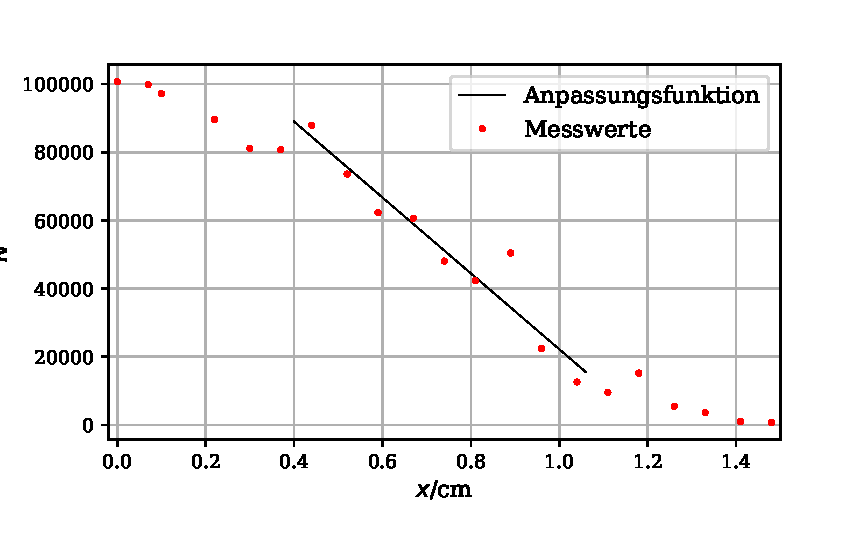
\includegraphics{plot2.pdf}
  \caption{Zählrate in Abhängikeit der effektiven Weglänge für einen Abstand von $1,5$ $\si{\cm}$. }
  \label{fig:plot}
\end{figure}

\subsection{Bestimmung des Energieverlustes}
Die berechneten Energien aus der ersten Messung werden gegen die effektive Weglänge aufgetragen. 
\begin{figure}[H]
  \centering
  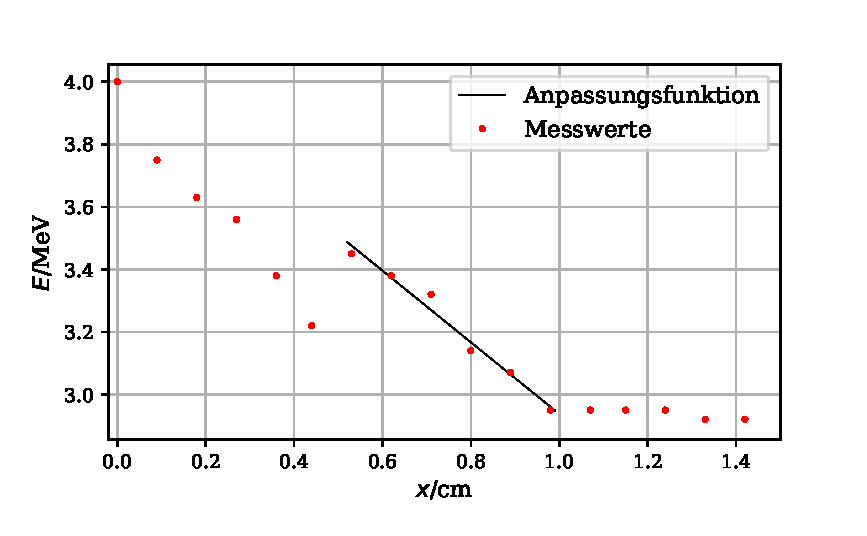
\includegraphics{plot3.pdf}
  \caption{Energie in Abhänigkeit der effektiven Weglänge für einen Abstand von $1,8$ $\si{\cm}$. }
  \label{fig:plot}
\end{figure}
\noindent Es wird erneut eine lineare Ausgleichsrechnung mit dem linearen Teil der Kurve durchgeführt. Der Energieverlust $-\frac{dE}{dx}$
liest sich als Steigung der Geraden ab, und beträgt somit
\begin{align*}
-\frac{dE}{dx} = (-1,14 \pm 0,09) \symup{\frac{MeV}{cm}} .
\end{align*}


\subsection{Statistik des radioakiven Zerfalls}

Es werden 100 Werte für die Zerfälle pro Zeiteinheit gemessen und notiert. Diese sind in Tabelle 3 zu finden.
\begin{table}[H]
  \centering
  \caption{Zerfälle pro Zeiteinheit.}
  \label{tab:Parameter}
  \begin{tabular}{c c c c c}
    \bottomrule
     5686&5855 &5500&5632&5605 \\
     5643&5855 &5725   &5112&5533 \\
     5280&5961  &5581  &5280&5069 \\
     5423&5540  &5739  &5224 &5095 \\
     5202&5755  &5726  &5035 &5357 \\
     5409&5644  &5856  &5654   &5371 \\
     5273&5804  &5929  &5272     &5416 \\
     5207&5675  &5862  &5356     &5553 \\
     5100&5444  &5688  &5219     &4978 \\
     5230&5910  &5820  &5424     &5523 \\
     5668&5961  &5234  &5099     &5195 \\
     5604&5952  &5567  &5373     &5590 \\
     5274&5795  &5070  &5178     &5207 \\
     5814&5319  &5090  &5184     &5187 \\
     5774&5506  &5503  &5006     &5204 \\
     5955&5267  &5705  &5317     &4949 \\
     5701&5496  &5526  &5510 &5455 \\
     5447&5784  &4991  &5189     &5540 \\
     5748&5560  &4991  &4983     &5126 \\
     6019&5512  &5439  &5171     &5516 \\
  \bottomrule
  \end{tabular}
\end{table}

\noindent Aus diesen Werten wird der Mittelwert und die Standardabweichung bestimmt
\begin{align*}
Z &= \frac{1}{100}\cdot \sum_{n=1}^{100} Z_i = 5462.81 \\
\Delta Z &=\frac{1}{\sqrt{100}} \cdot \sqrt{\frac{1}{99} \sum_{n=1}^{100} (Z_i - Z)^2} = 280,44.
\end{align*}

\noindent Außerdem wird die Varianz berechnet
\begin{align*}
Var(N) = 78647,35 .
\end{align*}
Die Messwerte werden in einem Histogramm aufgetragen
\begin{figure}[H]
  \centering
  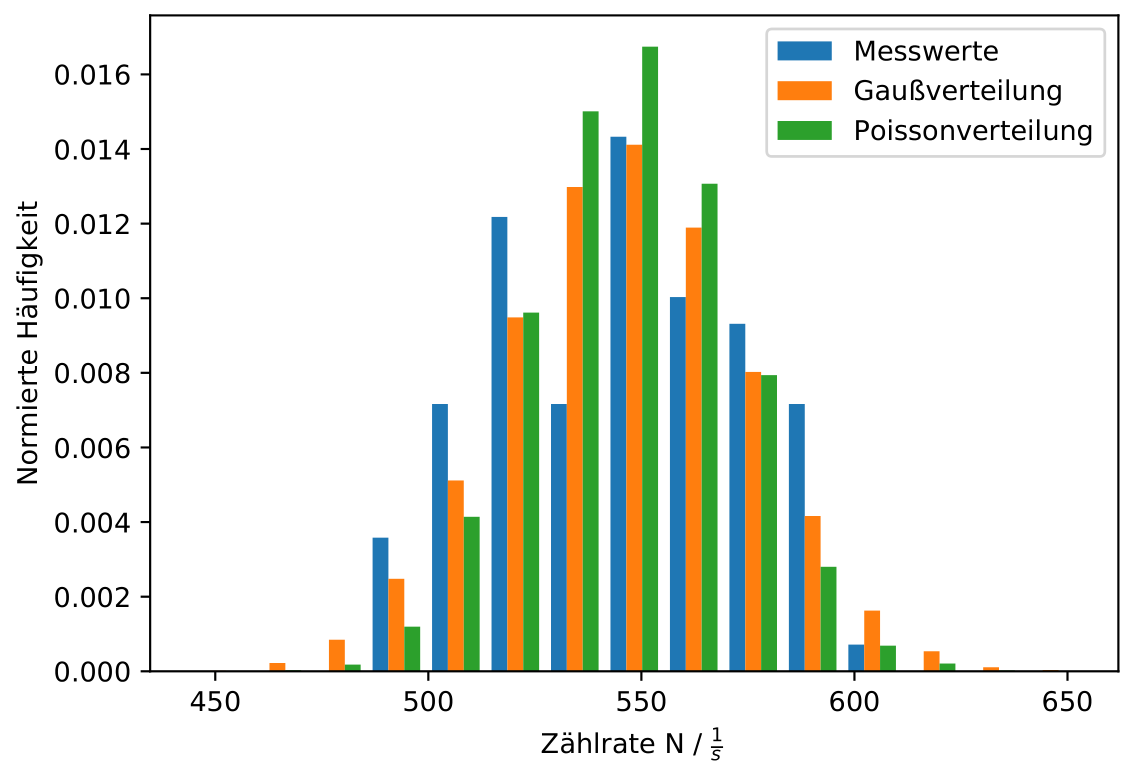
\includegraphics[width=0.8\textwidth]{h.PNG}
  \caption{Histogramm für die 100 Zählraten und Vergleich mit einer Poisson- und Gaußverteilung. }
  \label{fig:plot}
\end{figure}
\noindent Vergleicht man die berechneten Größen miteinander, so fällt auf, dass
das Quadrat der Standardabweichung ungefähr der Varianz entspricht. Deshalb kann bei diesen Messwerten gesagt werden, dass sie besser zu einer Gaußverteilung passen.

